%! TEX root = **/000-main.tex

\section{Bayesian Computation}

In Bayesian statistics, we must always calculate the posterior
distribution $\pi(\theta \mid y)$:

\begin{equation*}
	\pi(\theta \mid y) = \frac{L_y(\theta)p(\theta)}{\int L_y(\theta)p(\theta)\,d\theta}
\end{equation*}

The integral in the denominator is usually intractable analytically. For example, if
$\theta$ is a vector $\left(\theta_1,\,\theta_2,\,\dots,\,\theta_p \right)$,
the integral is a multidimensional integral:

\begin{equation*}
	\int L_y(\theta)p(\theta)\,d\theta = \int_{\Omega_p} \int_{\Omega_{p-1}} \cdots \int_{\Omega_1} L_y(\theta)p(\theta)\,d\theta_1\,d\theta_2\,\dots\,d\theta_p
\end{equation*}

Therefore, we must resort to numerical methods that simulate values from the posterior
distribution.
We call these methods \iemph{Bayesian computation}.

\subsection{Markov Chain Monte Carlo}

The MCMC algorithms allows us to simulate values from the posterior distribution given
a Bayesian model and Data.

The most common MCMC algorithms are:
\begin{itemize}
	\item Gibbs Sampling
	\item Metropolis Hasting
	\item Hamiltonian Monte Carlo
\end{itemize}

Given an initial value $\theta^{(0)}$, the MCMC algorithms generate a sequence of successive values
$\theta^{(1)},\,\theta^{(2)},\,\dots,\,\theta^{(n)}$. After a burn-in period, the values
$\theta^{(n)}$ are assumed to be independent and identically distributed (i.i.d.) from the
posterior distribution $\pi(\theta \mid y)$ (the chain has converged).

We can use the values after the burn-in period as simulations from the posterior distribution.
Therefore, we need to make sure that the chain has converged.

\subsubsection{Checking the convergence}

The convergence check can be done graphically by starting two (or more) chains
from different initial values and plotting the values of the chain. If the
chains have converged, the values of the chains should be similar.

Additionally, we must check that there is no autocorrelation in the chain.

If the chains have not converged, we should increase the number of iterations.

\begin{figure}[H]
	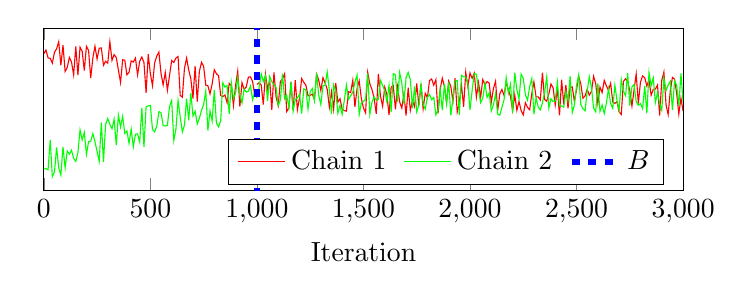
\begin{tikzpicture}
		\begin{axis}[
				samples at={0,10,...,3000},
				width=0.8\textwidth,
				height=0.3\textwidth,
				ytick=\empty,
				xmin=0,
				xmax=3000,
				xlabel={Iteration},
				legend pos=south east,
                xtick={0,500,1000,1500,2000,2500,3000},
                legend columns=-1,
                legend style={/tikz/every even column/.append style={column sep=0.4em}}]
			]
            \addplot[mark=none,color=red,samples at={0,10,...,1000}]
                {rand*10 - x*0.02+50}; \addlegendentry{Chain 1 };
            \addplot[mark=none,color=green,samples at={0,10,...,1000}]
                {rand*10 + x*0.03}; \addlegendentry{Chain 2 };
            \addlegendimage{dashed,blue,line width=2pt};
            \addlegendentry{$B$};

            \addplot[mark=none,color=red,samples at={1000,1010,...,3000}]
                {30 + rand*10};
            \addplot[mark=none,color=green,samples at={1000,1010,...,3000}]
                {30 + rand*10};
            \draw[dashed,blue,line width=2pt] (1000,-100) -- (1000,100);
		\end{axis}
	\end{tikzpicture}
    \caption{Example of two chains that converge at iteration $B = 1000$}
\end{figure}

The point $B$ is the iteration where the chains converge. We should set the burn-in parameter
to a number greater than $B$.

\subsubsection{JAGS}

JAGS is a software package for Bayesian analysis that uses MCMC algorithms.
It is written in C++ and has an R interface.
It allows us to specify a Bayesian model using a simple language (BUGS) and
it automatically generates the code for the MCMC algorithms.

Additionally, we can set the starting points of the chains, the number of chains,
the number of iterations, the burn-in period and the thinning factor.
The thinning factor allows us to reduce the autocorrelation in the chain
by only keeping every $n$ values.

\begin{recap}{Bayesian Computation}{}
	\begin{itemize}
		\item MCMC algorithms allow us to simulate values from the posterior distribution
		      starting from the Bayesian model and the data.
		\item We \emph{must} check the convergence of the chains before making any inference.
	\end{itemize}
\end{recap}



